\section{Grandezze e unità di misura}\label{sec:unita-di-misura}
Gli ordini di grandezza tipici delle strutture studiate dall'astrofisica rendono necessario introdurre delle nuove unità di misura rispetto a quelle standard.

\subsection{Lunghezze e massa}
Di seguito sono elencate le unità di misura maggiormente utilizzate per esprimere le lunghezze e le masse in astrofisica.
\begin{description}
    \item[Raggio solare] Vale $\si{\solarradius} \simeq \SI{6.7e10}{cm}$. Nella tabella~\ref{tab:ordini-grandezza-dimensioni-stelle} sono riportate le dimensioni di alcune stelle, espresse in raggi solari. Questa unità di misura viene utilizzata principalmente per esprimere la distanza di stelle e pianeti.
    \item[Unità astronomica] Esprime la distanza media tra Terra e Sole. Vale $\SI{1}{AU} \simeq \SI{1.5e13}{cm}$. Si utilizza principalmente per indicare distanze riferite al sistema solare e dintorni.
    \item[Anno luce] Rappresenta la distanza che la luce percorre nel vuoto in un anno, si utilizza molto nei libri di divulgazione scientifica ma non in ambito professionale. Vale $\SI{1}{ly} \sim \SI{9.5e17}{cm}$.
    \item[parsec] Indica la distanza alla quale $\SI{1}{AU}$ sottende un angolo di $\ang{;;1}$ (\emph{secondo d'arco}), come mostrato in figura~\ref{fig:parsec}. Vale $\SI{1}{pc} = \SI{3.1e18}{cm}$. Nella tabella~\ref{tab:ordini-grandezza-dimensioni-stelle} sono riportate le dimensione di alcune strutture cosmiche. Questa unità di misura si utilizza principalmente in astrofisica galattica ed extra--galattica.
    \item[Redshift] Viene utilizzato per indicare distanze dell'universo lontano e in cosmologia.
    \item[Massa Solare] Vale $\si{\solarmass} = \SI{2e33}{g}$. In tabella~\ref{tab:masse-solari} sono presenti alcuni valori tipici di massa.
\end{description}

\begin{table}
    \caption{Dimensioni di alcune stelle e strutture cosmiche.}
    \label{tab:ordini-grandezza-dimensioni-stelle}
    \centering
    \begin{tabular}{ll@{\qquad}ll}
        \toprule
        \multicolumn{2}{c}{Ordini di grandezza per le stelle} & \multicolumn{2}{c}{Ordini di grandezza per alcune strutture stellari} \\
        Stella & Dimensioni & Struttura & Dimensioni \\
        \midrule
        Giove & $\sim \SI{0.1}{\solarradius}$ & Galassie & $\sim \textup{qualche} \, \si{kpc}$ \\
        Giganti rosse & $\sim \SI{2000}{\solarradius}$ & Via Lattea & $\sim \SI{25}{kpc}$ \\
        Nane bianche & $\sim \SI{6000}{km}$ & Ammassi di Galassie & $\sim \textup{qualche} \, \si{Mpc}$  \\
        Stelle di neutroni & $\sim \SI{10}{km}$ & Nubi di Magellano & $\sim \SI{60}{kpc}$  \\
        \bottomrule
        \end{tabular}
\end{table}

\begin{table}
\caption{Masse di alcune strutture cosmiche.}
\label{tab:masse-solari}
\centering
\begin{tabular}{ll}
\toprule
Struttura & Massa (\si{\solarmass}) \\
\midrule
Stelle          & $0.08$--$150$ \\
Ammassi stellari           & $10^3$--$10^6$    \\
Galassie            & $10^7$--$10^{13}$  \\
Ammassi di galassie & $10^{14}$--$10^{15}$  \\
\bottomrule
\end{tabular}
\end{table}

\begin{figure}
    \centering
    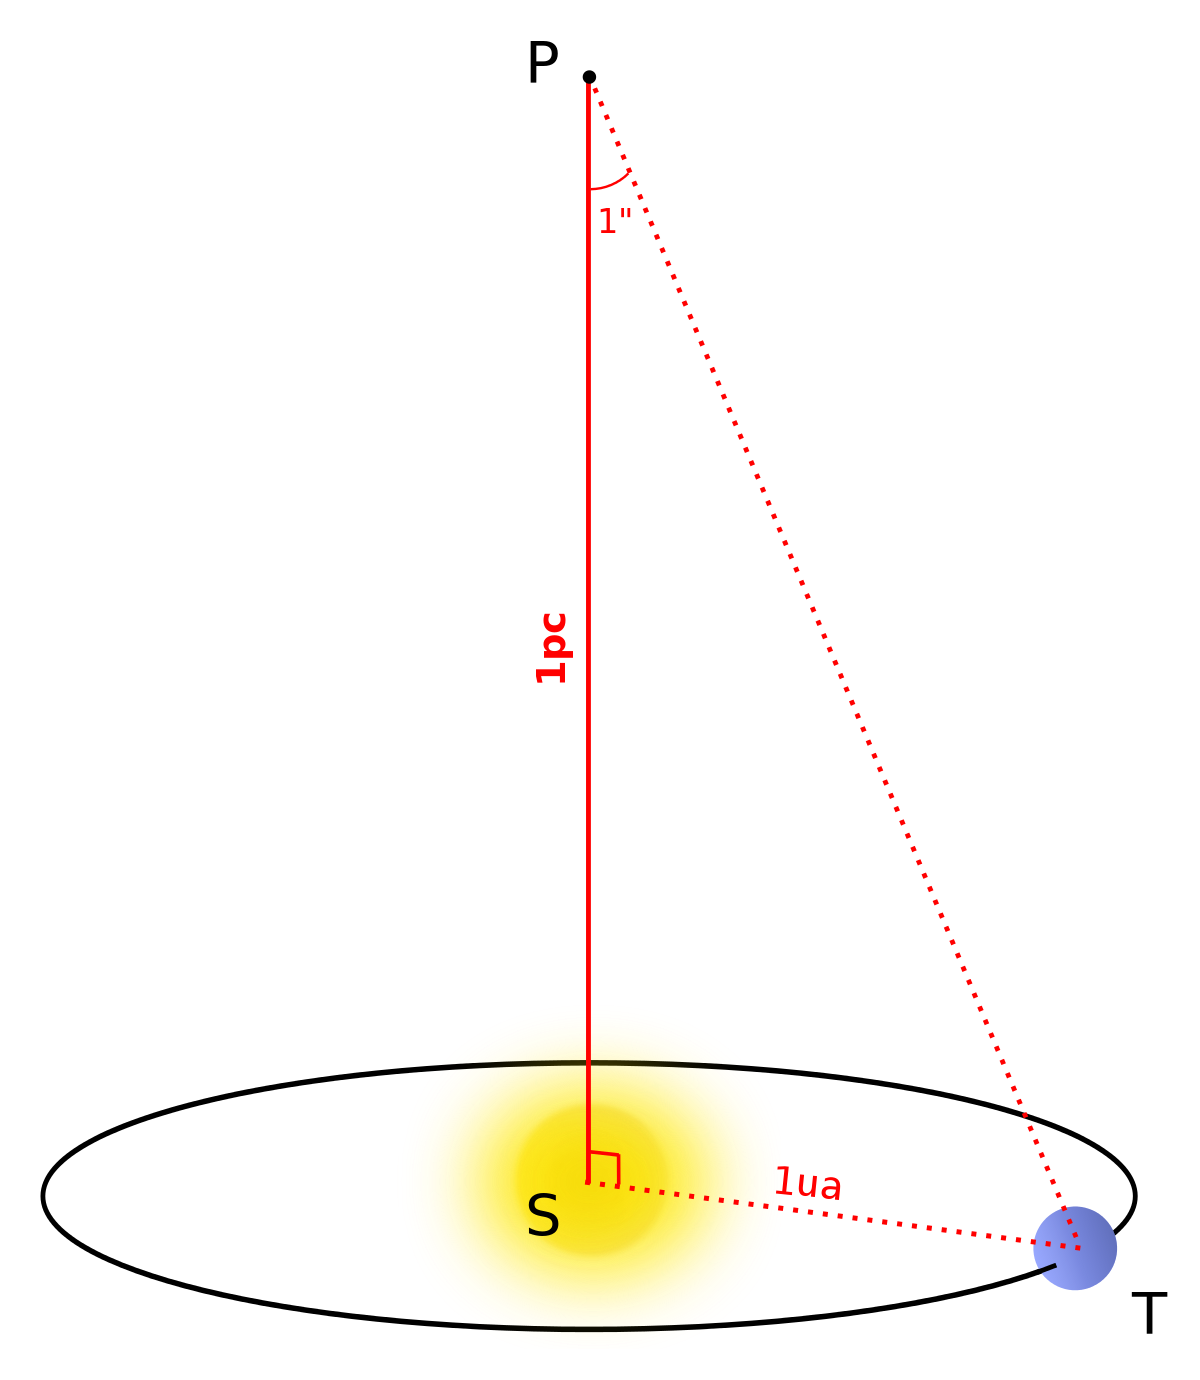
\includegraphics[width=0.3\textwidth]{immagini/parsec.png}
    \caption{Definizione di parsec. $\SI{1}{pc}$ è la distanza alla quale $\SI{1}{AU}$ sottende un angolo di $\ang{;;1}$.}
    \label{fig:parsec}
\end{figure}

\subsection{Sfera celeste}\label{sec:posizione-sfera-celeste}
Come anticipato precedentemente, non siamo in grado di osservare la profondità degli oggetti cosmici, ma solo la loro proiezione sulla \emph{sfera celeste}. Questa è, per definizione, una sfera di raggio indeterminato (per convenzione si pone $R=1$) centrata nell'osservatore (come mostrato in fig.~\ref{fig:sfera-celeste}). In genere, a seconda della convenienza, si considera il centro della sfera celeste coincidente con il \emph{centro della Terra} (sfera geocentrica), con il \emph{centro del Sole} (sfera eliocentrica) oppure con il \emph{baricentro del sistema solare} (sfera baricentrica). Se la distanza del corpo che si sta studiando è grande, scegliere uno dei tre centri è del tutto equivalente. Si definisce \emph{equatore celeste} la proiezione dell'equatore terrestre sulla sfera celeste e non è altro che un cerchio massimo. Si definisce \emph{asse del mondo} la retta passante per il centro $O$ della sfera celeste e perpendicolare al piano equatoriale. L'intersezione tra questa retta e la sfera celeste individua due punti detti \emph{poli celesti}: attualmente il polo nord celeste è circa nella direzione della stella polare, mentre il polo sud celeste è vicino alla croce del sud. 

L'\emph{eclittica} è definita come il cerchio massimo descritto dalla traiettoria (apparente) del sole attorno alla Terra, ovvero è l'intersezione tra la sfera celeste e il piano orbitale della Terra attorno al Sole. Essa è inclinata di $\ang{23;27;}$ rispetto all'equatore celeste e interseca l'equatore in due punti opposti, detti \emph{equinozi}: il \emph{punto della Bilancia} e il \emph{punto dell'Ariete} (o \emph{punto vernale} o \emph{equinozio di primavera}).

\begin{figure}
\centering
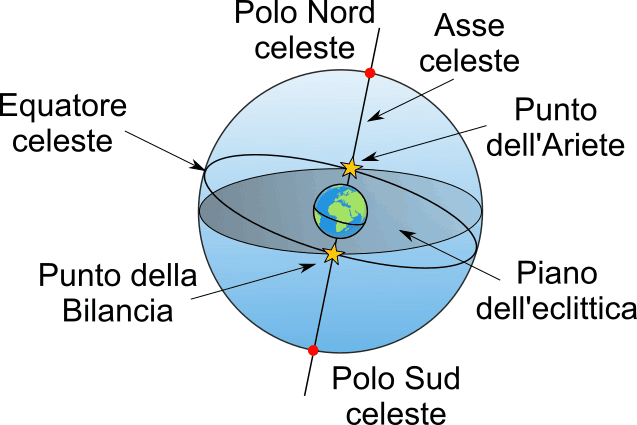
\includegraphics[width=0.5\textwidth]{immagini/sfera-celeste.png}
\caption{Sfera celeste. L'eclittica è l'intersezione tra la sfera celeste e il piano orbitale della Terra attorno al Sole. Essa interseca l'equatore terrestre in due punti opposti detti equinozi. Il punto dell'Ariete corrisponde all'equinozio di primavera (21 marzo), detto anche punto vernale.}
\label{fig:sfera-celeste}
\end{figure}

Lo \emph{Zenith} (fig.~\ref{fig:zenith}) è la congiungente tra il centro della Terra e l'osservatore, cioè la verticale dell'osservatore stesso. L'\emph{orizzonte astronomico} è il cerchio massimo formato dall'intersezione tra la sfera celeste e il piano perpendicolare alla verticale dell'osservatore. Ovviamente, l'osservatore è in grado di vedere solamente ciò che si trova sopra all'orizzonte astronomico. Si noti che lo Zenith e l'orizzonte astronomico dipendono dalla posizione dell'osservatore sulla Terra.

\begin{figure}
\centering
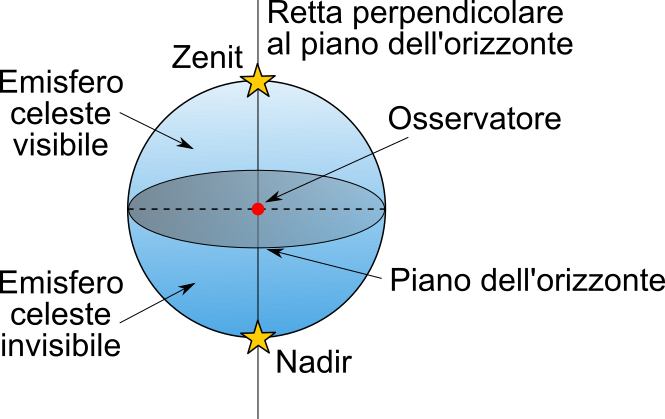
\includegraphics[width=0.5\textwidth]{immagini/zenit.png}
\caption{Zenith e orizzonte astronomico. L'osservatore vede solo ciò che sta sopra l'orizzonte astronomico. Dipendono da dove è posizionato l'osservatore sulla Terra.}
\label{fig:zenith}
\end{figure}

In ogni punto della Terra, l'osservatore la vede ruotare attorno all'asse del mondo, che passa per i \emph{poli celesti}, di cui solamente uno è visibile sopra all'orizzonte (cfr. fig.~\ref{fig:sfera-celeste}). Il moto delle stelle, rappresentato in fig.~\ref{fig:movimento-stelle} avviene da est verso ovest ed è un moto rigido attorno all'asse del mondo. Le distanze relative tra le stelle ci appaiono fisse, ciononostante ogni stella si muove di moto proprio, ma, data la distanza, le variazioni di posizione non sono apprezzabili. Il periodo di rotazione delle stelle definisce il così detto \emph{giorno siderale}.

\begin{figure}
\centering
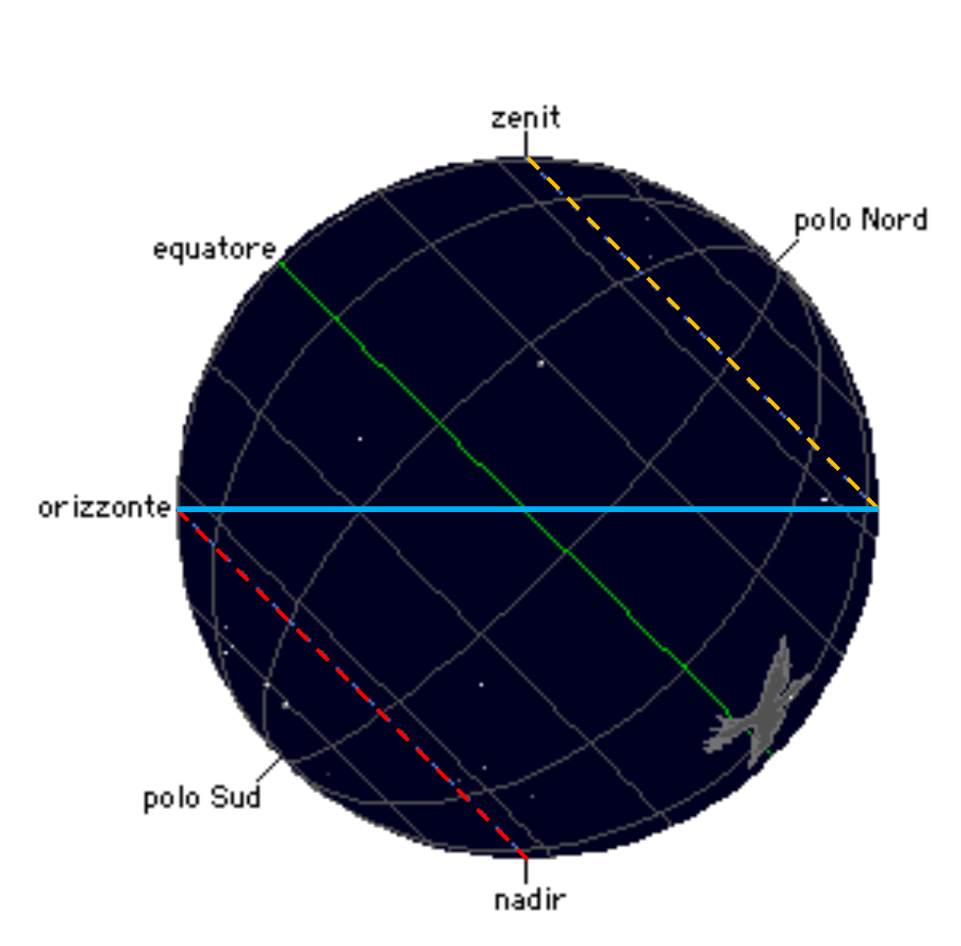
\includegraphics[width=0.3\textwidth]{immagini/movimento-stelle.png}
\caption{Come ci appare il movimento delle stelle. Tutte le stelle sopra il cerchio giallo non tramontano mai, quelle sotto il cerchio rosso non sorgono mai e le altre stelle le vediamo sorgere e tramontare.}
\label{fig:movimento-stelle}
\end{figure}

\subsection{Sistema equatoriale}
Come definire un sistema di coordinate sulla sfera celeste? Si ricordi che noi osserviamo delle proiezioni su un piano, quindi sono sufficienti due coordinate. In particolare, conviene utilizzare delle coordinate angolari e il sistema di coordinate più utilizzato è il \emph{sistema equatoriale} (fig.~\ref{fig:sistema-equatoriale}). Esso usa come cerchi di riferimento l'equatore celeste e il meridiano\footnote{Un meridiano è un cerchio massimo perpendicolare all'equatore.} passante per il punto vernale ($\gamma$). Chiamato $C$ il centro della sfera celeste, l'origine del sistema di coordinate è nel punto vernale, $O \equiv \gamma$, e ha per coordinate angolari l'ascensione della retta ($\alpha$) e la declinazione:
\begin{description}
    \item[Ascensione retta (RA o $\alpha$)] distanza angolare tra il punto $\gamma$ e il meridiano dell'astro. Si misura in ore, minuti e secondi (hms), varia tra $0^h$ e $24^h$, aumentando verso E.
    \item[Declinazione (Dec o $\delta$)] distanza angolare tra l'equatore celeste e l'astro, lungo il meridiano dell'astro. Si misura in gradi, primi e secondi (gradi, arcominuti e arcosecondi), varia tra $\ang{0}$ e $+\ang{90}$ dall'equatore al polo N e tra $\ang{0}$ e $-\ang{90}$ dall'equatore al polo S.
\end{description}
Si faccia attenzione al fatto che i minuti e secondi d'orologio (RA) sono \emph{diversi} dai minuti e secondi d'arco (Dec). Utilizzando:
\[
    1^h = 60^m = 3600^s \qquad \ang{1} = 60' = 3600'' \qquad 24^h = \ang{360}
\]
si trova che:
\[
    1^h = \ang{15} \qquad 1^m = 15' \qquad 1^s = 15''
\]

\begin{figure}
\centering
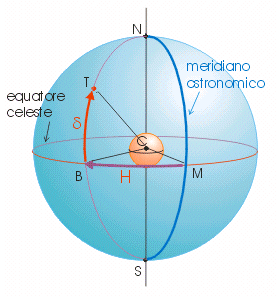
\includegraphics[width=0.3\textwidth]{immagini/sistema-equatoriale.png}
\caption{Sistema equatoriale. $C$ è il centro della sfera celeste, l'origine del sistema di riferimento coincide con il punto vernale, $O \equiv \gamma$. $\alpha$ è l'ascensione retta, ovvero la distanza angolare tra il punto $\gamma$ e il meridiano dell'astro, il quale, nella figura, interseca l'equatore celeste nel punto $B$. $\delta$ è la declinazione, ovvero la distanza angolare tra l'equatore celeste e l'astro, lungo il meridiano dell'astro. Nella figura corrisponde alla distanza angolare tra $B$ e la stella.}
\label{fig:sistema-equatoriale}
\end{figure}

Si guardi la figura~\ref{fig:esempio-sistema-equatoriale} per un esempio sull'utilizzo di tale sistema di coordinate.

\begin{figure}
\centering
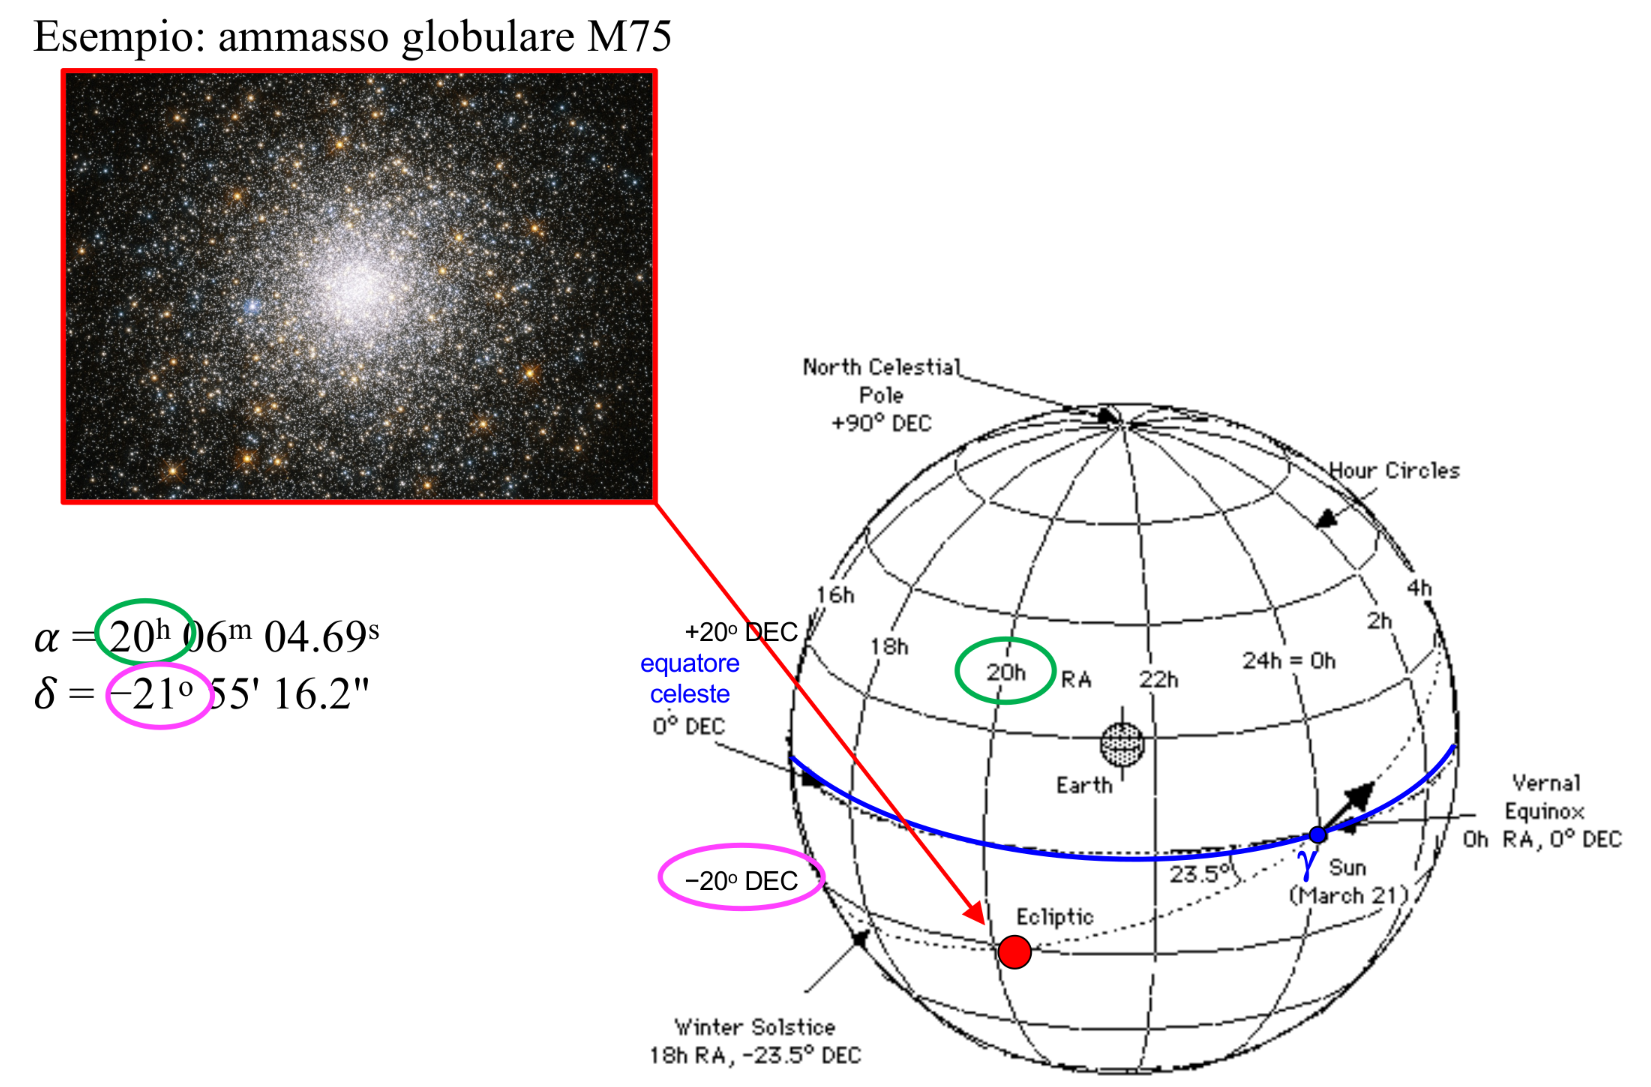
\includegraphics[width=0.5\textwidth]{immagini/esempio-sistema-equatoriale.png}
\caption{Esempio di utilizzo delle coordinate del sistema equatoriale.}
\label{fig:esempio-sistema-equatoriale}
\end{figure}